\documentclass[dvipdfmx]{standalone}
\usepackage{tikz}
\usepackage{amssymb} % \square用

\begin{document}

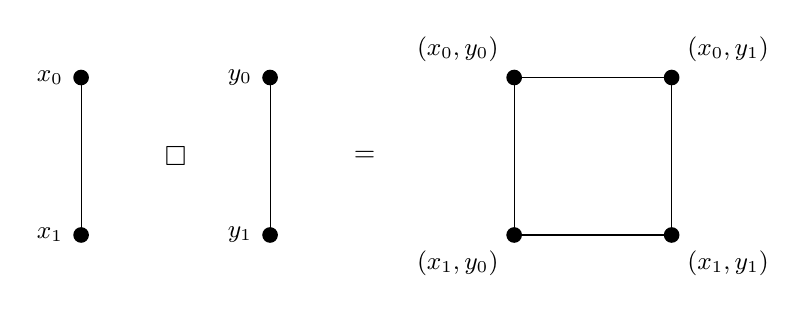
\begin{tikzpicture}
    % ==========================
    % 設定
    % ==========================
    \def\len{2.0} % 辺の長さ
    \tikzset{
        dot/.style={circle, fill=black, inner sep=2pt}, % 頂点のスタイル
        every label/.style={font=\small} % ラベルのフォントサイズ
    }

    % ==========================
    % 1. 左の C2 (x成分)
    % ==========================
    \begin{scope}[local bounding box=G1]
        \coordinate (x0) at (0, \len);
        \coordinate (x1) at (0, 0);

        \draw (x0) -- (x1);
        \node[dot, label=left:$x_0$] at (x0) {};
        \node[dot, label=left:$x_1$] at (x1) {};
    \end{scope}

    % 記号: square
    \node at (1.2, \len/2) {$\square$};

    % ==========================
    % 2. 真ん中の C2 (y成分)
    % ==========================
    \begin{scope}[xshift=2.4cm, local bounding box=G2]
        \coordinate (y0) at (0, \len);
        \coordinate (y1) at (0, 0);

        \draw (y0) -- (y1);
        \node[dot, label=left:$y_0$] at (y0) {};
        \node[dot, label=left:$y_1$] at (y1) {};
    \end{scope}

    % 記号: =
    \node at (3.6, \len/2) {$=$};

    % ==========================
    % 3. 右の C4 (直積グラフ)
    % ==========================
    \begin{scope}[xshift=5.5cm, local bounding box=G3]
        % 座標定義
        \coordinate (TL) at (0, \len);    % 左上
        \coordinate (TR) at (\len, \len); % 右上
        \coordinate (BL) at (0, 0);       % 左下
        \coordinate (BR) at (\len, 0);    % 右下

        % 辺の描画 (正方形)
        \draw (TL) -- (TR) -- (BR) -- (BL) -- cycle;

        % 頂点とラベル
        % 左上 -> (x0, y0)
        \node[dot, label=above left:{$(x_0, y_0)$}] at (TL) {};
        % 右上 -> (x0, y1)
        \node[dot, label=above right:{$(x_0, y_1)$}] at (TR) {};
        % 左下 -> (x1, y0)
        \node[dot, label=below left:{$(x_1, y_0)$}] at (BL) {};
        % 右下 -> (x1, y1)
        \node[dot, label=below right:{$(x_1, y_1)$}] at (BR) {};
    \end{scope}

\end{tikzpicture}

\end{document}